\documentclass{article}
\usepackage[utf8]{inputenc}
\usepackage{amsmath}
\usepackage{graphicx}

\begin{document}
\section{1.}
In our serial adder, we quite straightforwadly sum our vector recursively, from the back of the vector and stores the sum in the beginning. Please don't watch to closely on the inline version.

The results from the serial implementation:
\begin{verbatim}
s = 1.6449340668
s - 2^3 	 0.1175120147
s - 2^4 	 0.0605875334
s - 2^5 	 0.0307668040
s - 2^6 	 0.0155035654
s - 2^7 	 0.0077820619
s - 2^8 	 0.0038986305
s - 2^9 	 0.0019512189
s - 2^10 	 0.0009760858
s - 2^11 	 0.0004881621
s - 2^12 	 0.0002441108
s - 2^13 	 0.0001220629
s - 2^14 	 0.0000610333
\end{verbatim}

\section{}
Hmmm, yes it works. 

\section{Which MPI-calls are convenient / neccesary}
MPI_Send(...) and  MPI_Recv() were the only ones we used apart from the initialization calls. 
MPI_Reduce could be used instead of a for loop with MPI_Recv, which may have been more convenient than our solution.  

MPI_Init, MPI_Comm_size and MPI_Comm_rank were neccesary to get the info about the processes and make only one process do a given task. 
MPI_Get_processor_name were convenient we thought for following the process in more detail, but we never got different names from any run of the program, but from documentation this should have yielded a unique identifier of the process. 

\section{6}
No, they should not be the same in the sequential singleprocessor program and the multithreaded/multiprocessed versions. Taking the sum sequential could give troubles when the accumulated sum is getting to the point where we loose some precision when adding the next element. 

From a precision poitn of view the best way to add floating poitn numbers would be to put them on a min-heap and pop two, sum and push back to stack untill the stack contains one number. This howerver is rather inefficient ($n\log n $) and not really that much better than splitting into shorter arrays and doing each sequentially. 

By increasing the number of processes doing the sums of sequences we should get better precision and it seems we do when we look at the results, the error is being reduced if we increase the process/thread number. 

We  do however start to loose precision when we increase the process/thread count, due to 80-bit internal floating point registers on x86 we believe. That results in taking a sum out of the registers makes you possibly loose some precision opposed to just sequentially adding in these registers. 

All these things leads us to think that we should not have the same results for sequential, 2 processes and 8 processes. Although the math technically is the same it differs due to floating point representation. 

\section{7}
Since we generate and therefore hold it in memory on one process and copies parts of it to other processes we have a memory requirement which is $2^n\cdot\left(1-\frac{\text{nproc}-1}{\text{nproc}}\right)+\text{overhead}$. 

\section{8}
We concluded that $n^{-2}$ would require two floating point operations so generating it would require $2n$ operations. 

Assuming sequential operation: $3n = 2n+n$. Technically there is a minus one in there but it is insignificant. 

No, only one process does the work of generating the list, which is a significant part of the job. 

\section{9}
hell no! We paralellized the least intensive part of the program. 


\section{OpenMPI implementation }
Making an OpenMPI implementation we used the restrictions given in the assignment, which allow us to make a cleaner implementation. 

\begin{enumerate}

\item We do a number of iterations which is a power of two. 

\item We use a number of processes which is a power of two. 

\end{enumerate}

\begin{align}
2^{m}/2^{n} = 2^{m-n}
\end{align}

One effect of this is that we can partition the array, $2^{m}$ in the equation above, by dividing the size by the number of processes, $2^{n}$ above, to achieve the size of each partition, $2^{m-n}$. 
Since all these numbers can be represented as integers this gives no loss when doing integer division. 

We split the work into a few steps, populating the array, sending out the arrays to the workers, adding the elements of the arrays, sending back the answer, receiving the answer and summing the sums together. 

The primary thread is the only thread generating the array, it then sends all the other threads a piece of the array. 
Every other thread waits to receive its part. 
At this point every thread got one partition of the array, so they all find the sum of the contents in their partition. 
Every thread except the primary thread then proceeds to send the data back to the primary thread, which have been reveiving data from the threads and makes the final sum. 


\section{OpenMP and OpenMPI }
The differnce between the OpenMPI implementation and the combination is that the primary thread is using OpenMP to split the job into several senders and using the same technique for receiving. 
In addition the workers use OpenMP to paralellize their work. 


\begin{figure}
\caption{To achieve paralellization of reception we chose to use OpenMP's reduction in combination with {\tt MPI\_Receive}. This yields easy readable code which is paralellized. }
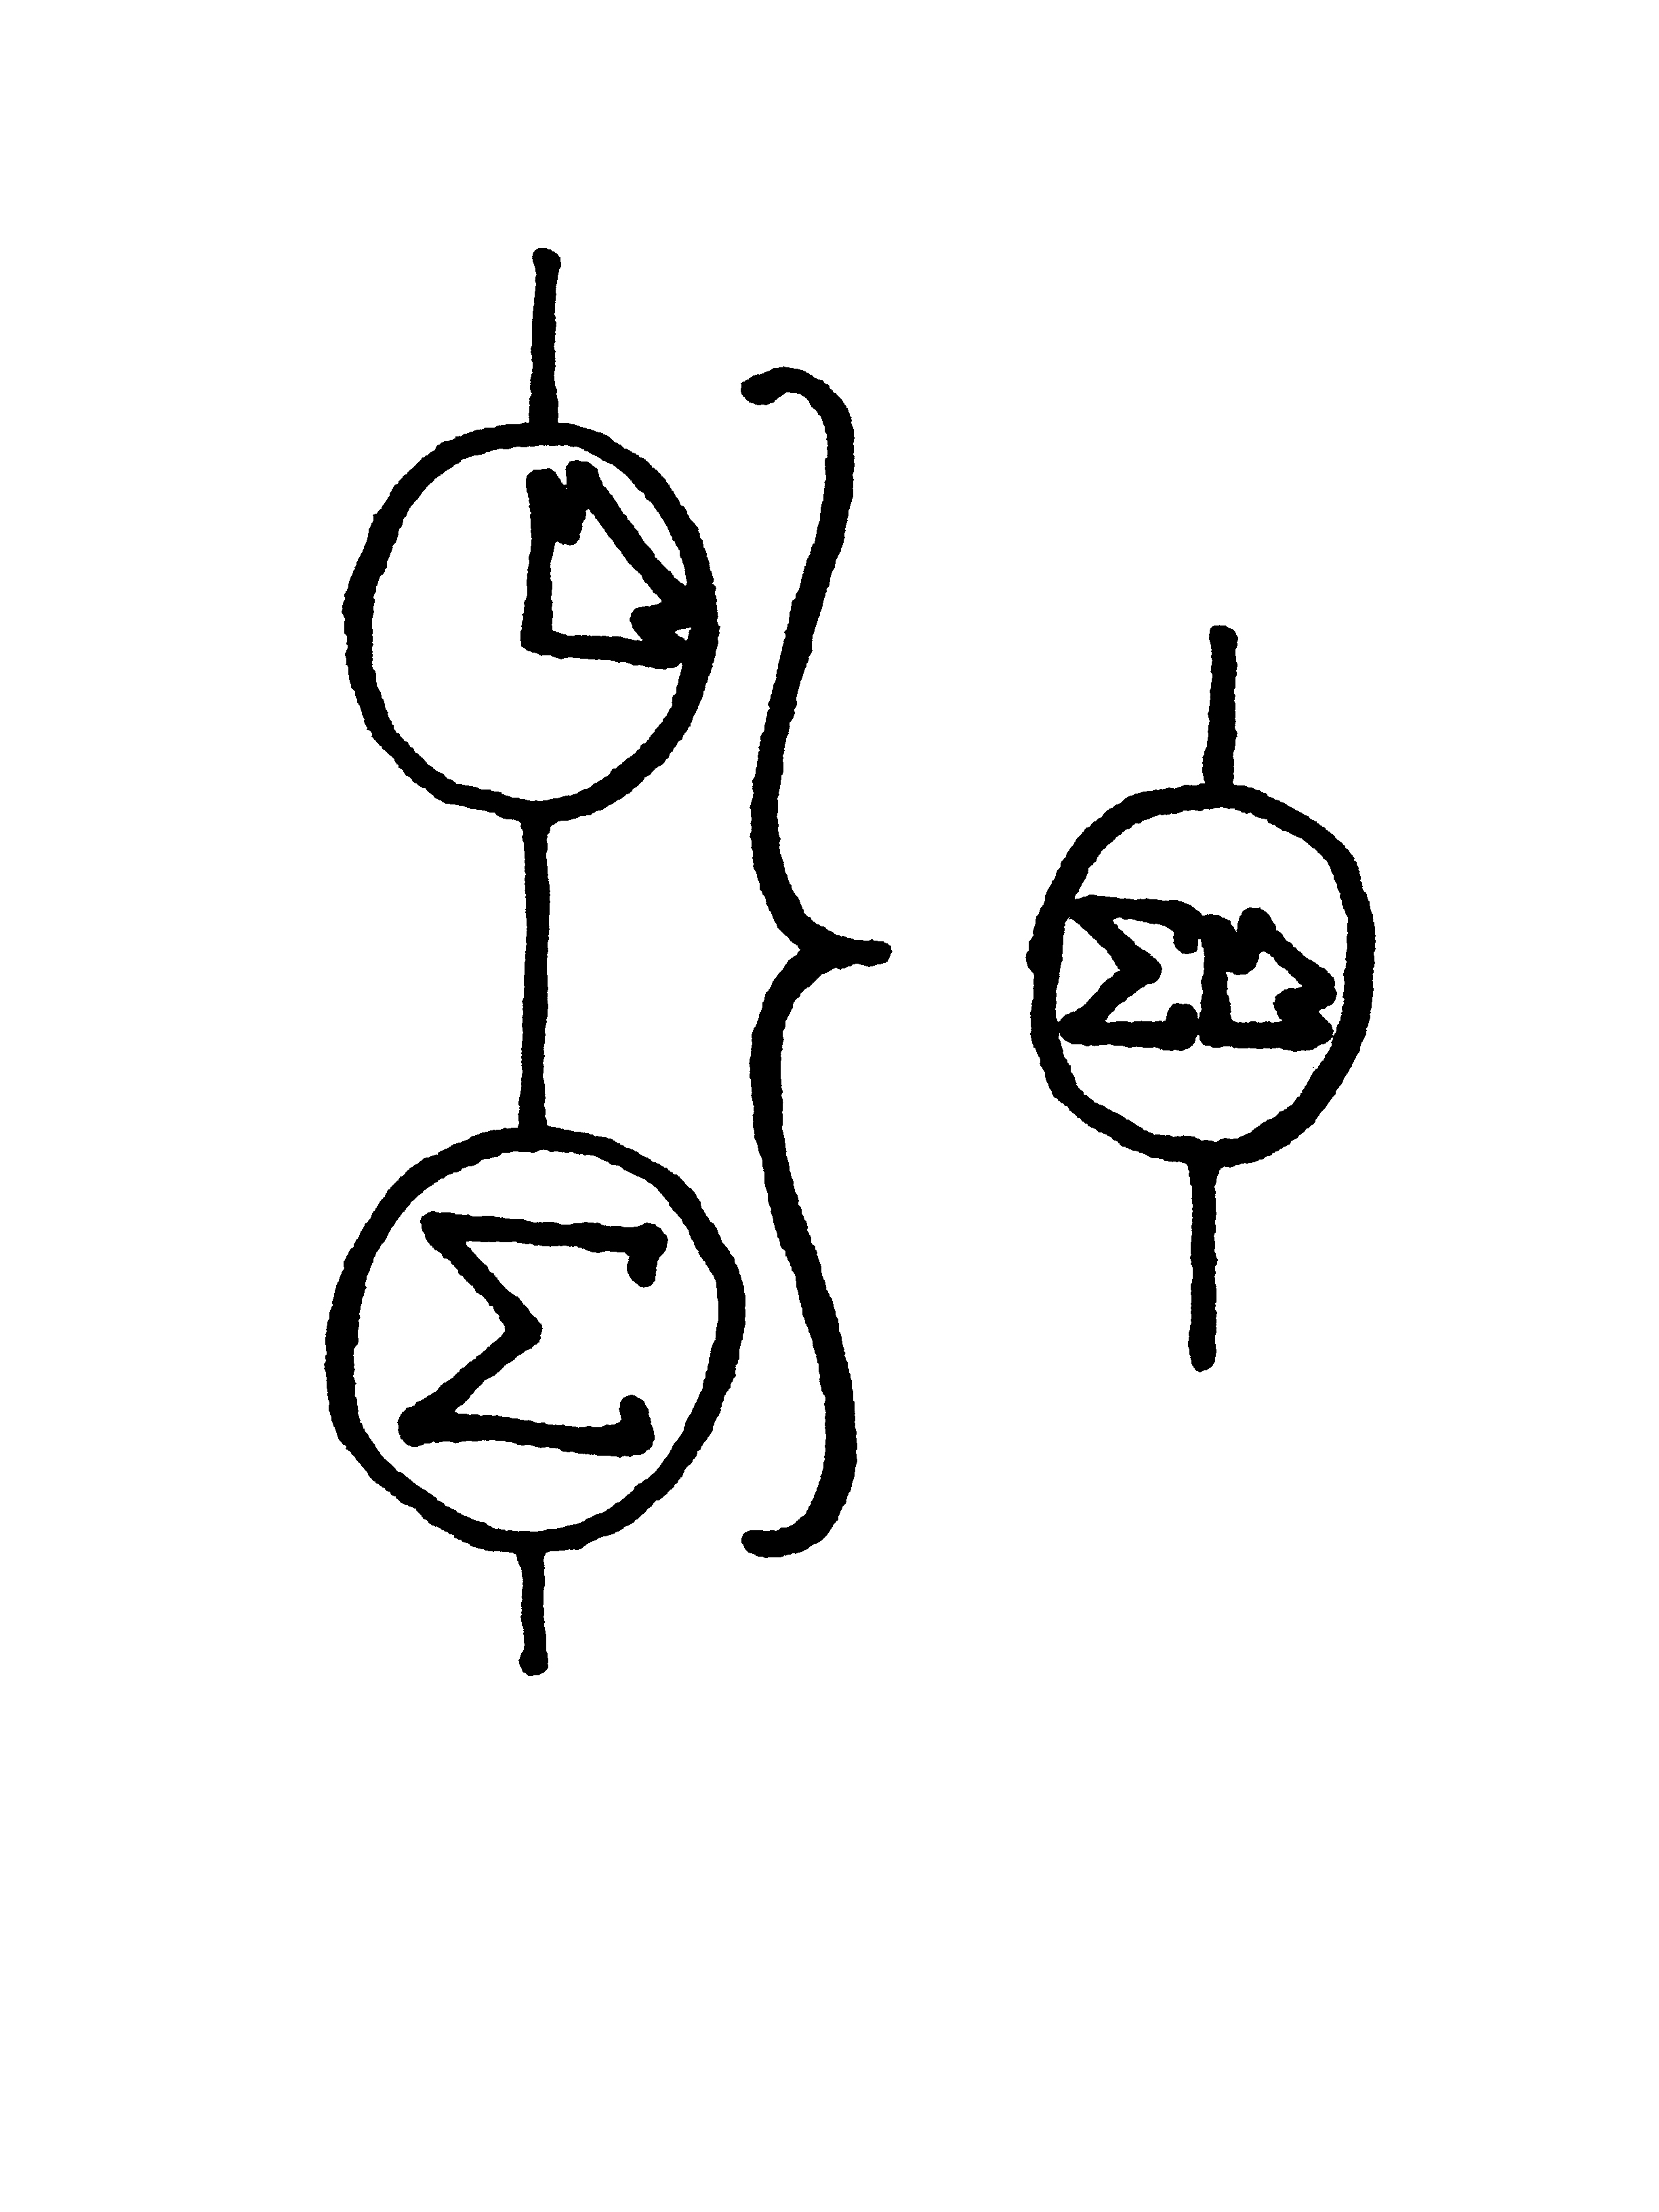
\includegraphics[width=\textwidth]{flyt2}
\end{figure}
\begin{figure}
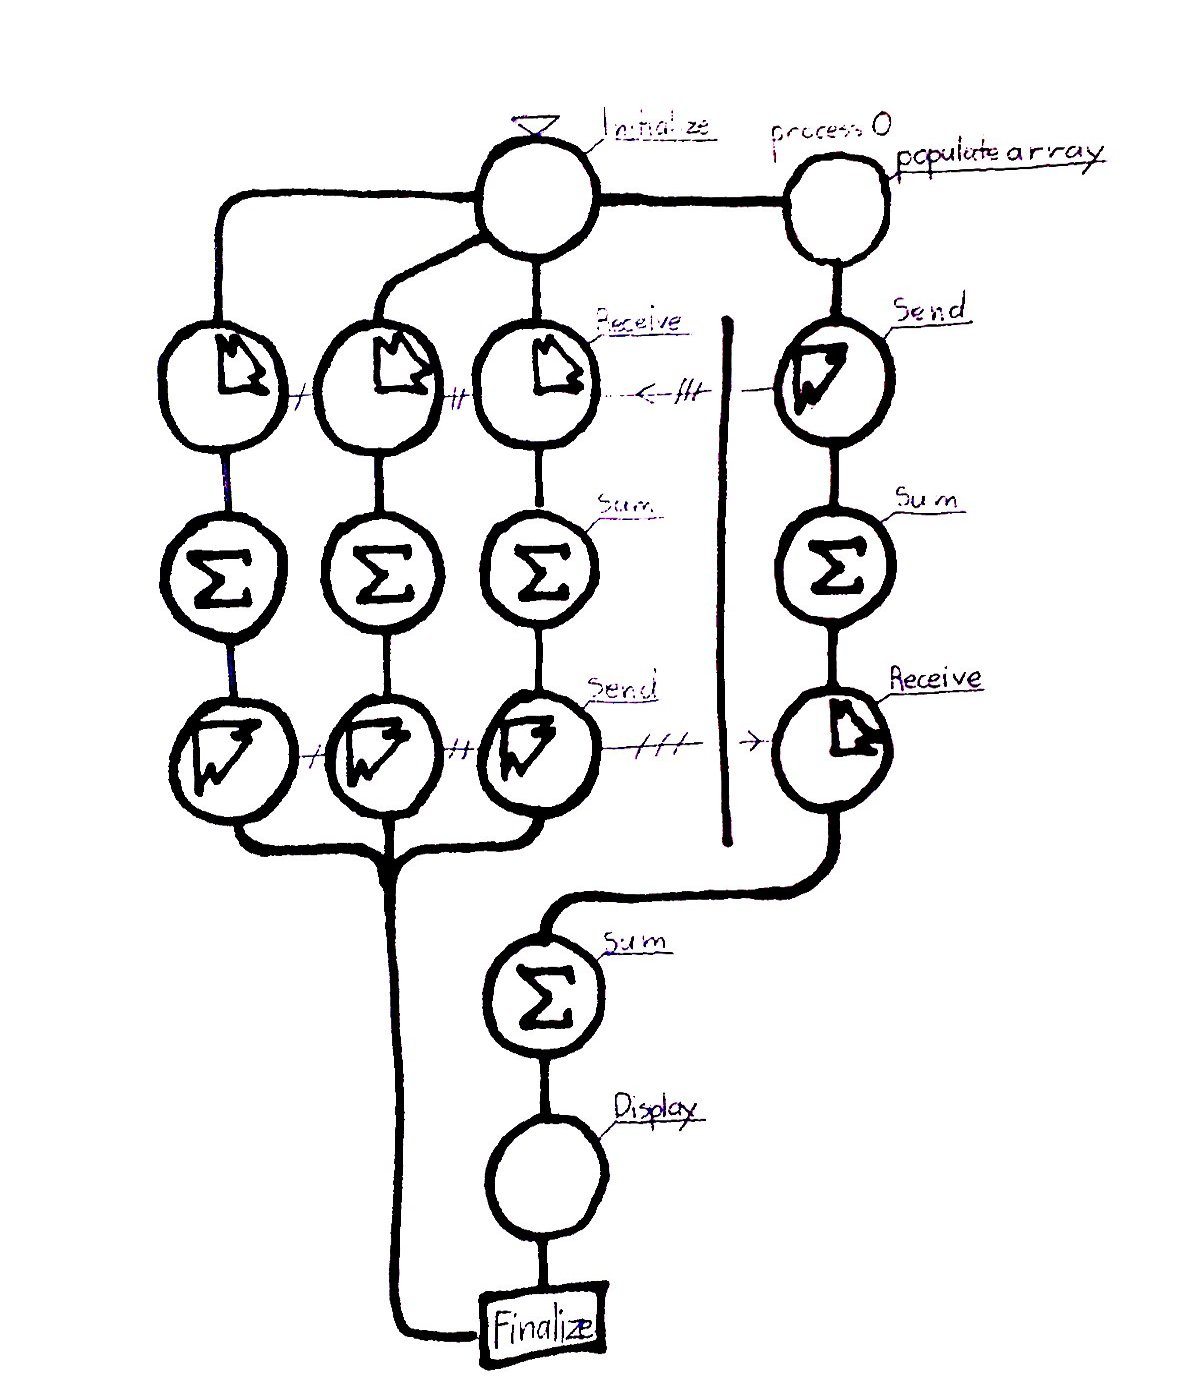
\includegraphics[width=\textwidth]{flytskjema1}
\caption{After each process is initiated and given rank, the primary process generates the full sequence alone. This is split into partitions, disjoint sets with full coverage, which is sent to each worker process. Each process, including the primary process will then take the sum of their sequence. Afterwards ay process not the primary one will proceed to send back the sum of its partition to the primary process which receives. The sums of the sums is then taken and displayed. }
\end{figure}



\end{document}
